%   ******Start of file apssamp.tex ******
%
%   This file is part of the APS files in the REVTeX 4.2 distribution.
%   Version 4.2a of REVTeX, December 2014
%
%   Copyright (c) 2014 The American Physical Society.
%
%   See the REVTeX 4 README file for restrictions and more information.
%
% TeX'ing this file requires that you have AMS-LaTeX 2.0 installed
% as well as the rest of the prerequisites for REVTeX 4.2
%
% See the REVTeX 4 README file
% It also requires running BibTeX. The commands are as follows:
%
%  1)  latex apssamp.tex
%  2)  bibtex apssamp
%  3)  latex apssamp.tex
%  4)  latex apssamp.tex


\documentclass[%
 reprint,
%superscriptaddress,
%groupedaddress,
%unsortedaddress,
%runinaddress,
%frontmatterverbose, 
%preprint,
%preprintnumbers,
nofootinbib,
%nobibnotes,
%bibnotes,
 amsmath,amssymb,
 aps,
%pra,
%prb,
%rmp,
%prstab,
%prstper,
%floatfix,
]{revtex4-2}

\usepackage{mycommands}

\begin{document}

\preprint{APS/123-QED}

\title{\axionbloch{}: an Open-Source Python Package for Simulating Axion-Induced Spin Dynamics}

\author{Yuzhe Zhang}
\email{Contact author: yuhzhang@uni-mainz.de}
\affiliation{Johannes Gutenberg-Universit{\"a}t Mainz, 55128 Mainz, Germany}
\affiliation{Helmholtz Institute Mainz, 55099 Mainz, Germany}
\affiliation{GSI Helmholtzzentrum für Schwerionenforschung GmbH, 64291 Darmstadt, Germany}

% \author{Derek F. Jackson Kimball}
% \affiliation{Department of Physics, California State University--East Bay, Hayward, CA 94542-3084, United States of America}

% \author{Alexander O. Sushkov}
% \affiliation{Department of Physics, Boston University, Boston, MA 02215, United States of America}
% \affiliation{Department of Electrical and Computer Engineering, Boston University, Boston, MA 02215, United States of America}
% \affiliation{Photonics Center, Boston University, Boston, MA 02215, United States of America}
% \affiliation{Department of Physics \& Astronomy, The Johns Hopkins University, Baltimore, MD 21218, United States of America}

% \author{Dmitry Budker}
% \affiliation{Johannes Gutenberg-Universit{\"a}t Mainz, 55128 Mainz, Germany}
% \affiliation{Helmholtz Institute Mainz, 55099 Mainz, Germany}
% \affiliation{GSI Helmholtzzentrum für Schwerionenforschung GmbH, 64291 Darmstadt, Germany}
% \affiliation{Department of Physics, University of California, Berkeley, CA 94720-7300, United States of America}

% \author{Hendrik Bekker}
% \affiliation{Johannes Gutenberg-Universit{\"a}t Mainz, 55128 Mainz, Germany}
% \affiliation{Helmholtz Institute Mainz, 55099 Mainz, Germany}
% \affiliation{GSI Helmholtzzentrum für Schwerionenforschung GmbH, 64291 Darmstadt, Germany}


% \author{Arne Wickenbrock}
% \affiliation{Johannes Gutenberg-Universit{\"a}t Mainz, 55128 Mainz, Germany}
% \affiliation{Helmholtz Institute Mainz, 55099 Mainz, Germany}
% \affiliation{GSI Helmholtzzentrum für Schwerionenforschung GmbH, 64291 Darmstadt, Germany}


% \collaboration{CASPEr Collaboration}

% \author{And more people? }

\begin{abstract}

% Ultralight bosonic dark matter with normal-matter spins can be described as the action of a pseudomagnetic field. 
The interaction of ultralight bosonic dark matter with spins can be interpreted as a pseudomagnetic field acting on normal matter.
Such interactions can be modeled like usual magnetic interactions using spin-evolution (Bloch) equations.
% Hypothetic beyond-standard-model interactions between axions and fermionic spins might induce magnetic signals. 
\axionbloch{}, an open-source Python package for simulating spin dynamics induced by both usual and exotic interactions, is presented. 
The numerical simulations serve as a tool for deriving axion signal signatures, which are crucial for designing experimental searches and data analysis. 
Simulations are calibrated against theoretical expectation, ensuring the accuracy of the simulated signals. 
\axionbloch{} is available at \url{https://github.com/Yuzhe98/AxionBloch}, allowing researchers to simulate axion pseudomagnetic signals under specific configurations of the axion models and experimental setups. 
The package is documented at \url{http://axionbloch.readthedocs.io/} and includes example scripts for application. 

\end{abstract}

\maketitle

\section{Introduction}

The axion was originally proposed to resolve the strong $CP$ problem in quantum chromodynamics\,\cite{PecceiQuinn1977_ConstraintsCP_PRD,Weinberg1978_NewLightBoson,PecceiQuinn1977_CPConservation_PRL,Wilczek1978_ProblemStrongPAndT}. 
Here $C$ denotes charge conjugation and $P$ denotes parity. 
Later, more general axionlike particles (ALPs) were proposed in various extensions of the Standard Model associated with spontaneously broken global symmetries\,\cite{svrcek2006axions,Kim1987_LightPseudoscalars,JaeckelRingwald2010_ALPReview,Arvanitaki2010_StringAxiverse}. 
Concerning the cosmological implications, axions and ALPs are also well-motivated dark matter candidates\,\cite{Preskill1983_invisible_axion,Abbott1983_CosmologicalBoundAxion,Marsh2016_AxionCosmology}.
In this paper, axions and ALPs are referred to as ``axions'' for simplicity. 

Axions may possess couplings to ordinary Standard Model particles\,\cite{Graham2013_Newobservables}, including photons, gluons and fermions. 
Crucially, axion field gradients ($\mathbf{\nabla}a$) may couple to fermionic spins through a pseudoscalar interaction. The Hamiltonian for this interaction can be expressed as
\begin{equation}
    \mathcal{H}_{\mathrm{int}} = - g_\mathrm{aNN} \mathbf{\nabla}a \cdot \mathbf{S}\,,
\end{equation}
where $g_\mathrm{aNN}$ is the axion-spin coupling strength, and $\mathbf{S}$ is the spin operator. 
The axion field gradient can be regarded as a pseudomagnetic field that mimics the behavior of a real magnetic field, where the Hamiltonian can be written as
\begin{equation}
    \mathcal{H} = -\hbar \gamma \mathbf{B} \cdot \mathbf{S} \,,
\end{equation} 
where $\gamma$ is the gyromagnetic ratio of the spin, and $\mathbf{B}$ is the magnetic field. 
The pseudomagnetic field induces spin dynamics, providing a pathway for detection in precision measurement experiments such as nuclear magnetic resonance (NMR) and comagnetometer-based searches\,\cite{ouellet2019first, du2018search, ALPHA2023,aja2022canfranc,CAPP2024,brouwer2022projected,alesini2023future,ZhongL2018results,garcia2024searchaxiondarkmatter,Quiskamp2024_ORGAN,rettaroli2024search,Gramolin2021_Ferromagnetic,gavilan2024searching,bloch2105nasduck,abel2023_HgDM,karanth2023first,LeeJunyi2023_NeutronSpin,capozzi2023new, CASPErProposal2014, kimball2018overview, wang2018application, aybas2021_SolidStateNMR, CASPEr_ZULF_2019,Walter2025_CASPErG}. 
There have been dedicated studies of the axion-induced spin dynamics\,\cite{Aybas_2021_Quantum_sensitivity, Dror2023_SensitivityAxion, Yuzhe2023_FrequencyScanning}, providing axion signal signatures and experimental sensitivity to axion fields. 
However, to our knowledge, there have not been studies taking advantage of numerical methods to verify the derived axion signal signatures. 
On the other hand, as more axion models and experiments are being proposed, such as cosmic axion background\,\cite{Dror2021_CosmicAxionBackground,Nitta2023_ADMX_CosmicAxionBackground}, fine-grained axion\,\cite{OHare2025_Finegrained}, and quadratically coupled axion\,\cite{GanXucheng2026_quadraticPTA, huang2026earthmatterenhancedaxion}, a tool is needed to systematically simulate the axion-induced spin dynamics under various physical conditions and axion field configurations.

In this work, \axionbloch{}, an open-source package designed to simulate spin dynamics induced by axion fields, is introduced. 
The interface is implemented in Python, a programming language known for its simplicity and readability, while the underlying numerical integration is implemented in C++ for efficiency. 
The package provides a flexible framework for modeling axion fields and experimental configurations. 
By numerically solving the relevant spin evolution equations, \axionbloch{} enables the prediction and analysis of experimentally observable signals.

%-----------------------
\section{Capabilities}
\label{sec:capabilities}
%-----------------------

In this section, the main components of \axionbloch{} are described. The section starts with the units, physical quantities, and constants (\cref{sec:units_quantities_constants}). Then, it continues with the physics and the algorithm for the numerical simulation (\cref{sec:algorithm}), after which the calibration for the simulation follows (\cref{sec:calibration}). In the end, an example simulation of axion-induced signals is provided (\cref{sec:simulation}). 


\subsection{Units, Physical Quantities, and Constants}


\label{sec:units_quantities_constants}

The packages takes advantage of \texttt{astropy}\footnote{\url{https://astropy.org/}}\,\cite{Astropy2013} to deal with units and physical quantities. 
Using \texttt{astropy.units}, physical quantities are created by attaching units to Python scalars or \texttt{NumPy}\footnote{\url{https://numpy.org/}}\,\cite{Harris2020_NumPy} arrays. 
Quantities can be converted between dimensionally equivalent units using the \texttt{to()} method.
In \texttt{astropy}, unit definitions are included in both the International System of Units (SI) and the Centimeter-Gram-Second (CGS) systems. 
Values in SI or CGS units can be found in the quantity's properties \texttt{.si} and \texttt{.cgs}.
A code example can be found in \cref{code:quantities}. 

In \texttt{axionbloch.constants}, a few commonly-used constants in axion and NMR research, such as gyromagnetic ratios, are defined.
The constants are instances of \texttt{astropy.units.Quantity}; therefore, all operations on physical quantities are supported for the constants. 

\begin{figure}
\center
\fbox{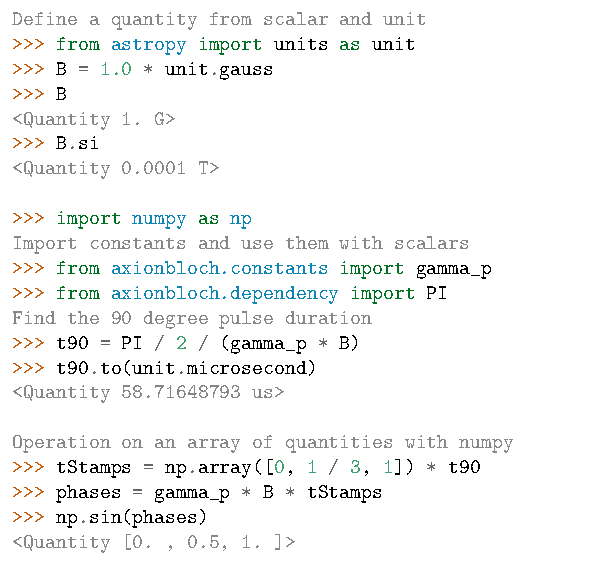
\includegraphics[scale=0.8,clip]{figures/code_quantities.pdf}}
% \vspace{0.1in}
\caption{Examples of operations of physical quantities using \texttt{astropy.units} and \texttt{axionbloch.constants}. }
\label{code:quantities}
\end{figure}

\subsection{Algorithm}
\label{sec:algorithm}

\subsubsection{Spin Dynamics}
\label{sec:spindynamics}

Considering the current experiments looking for axion-induced spin dynamics, \axionbloch{} focuses on spin-$1/2$ magnetic resonance. 
Different spins may be addressed in future updates. 
Magnetization is used as the observable to characterize the spin ensemble. 
In the presence of magnetic fields, including both bias fields applied in experiments and the axion-induced pseudomagnetic fields, the magnetization $\mathbf{M}$ evolves as
\begin{align}
\frac{d M_x}{dt} &= \gamma \left( \mathbf{M} \times \mathbf{B}_{\mathrm{eff}} \right)_x - \frac{M_x}{T_2}\,,\label{eq:bloch_x} \\
\frac{d M_y}{dt} &= \gamma \left( \mathbf{M} \times \mathbf{B}_{\mathrm{eff}} \right)_y - \frac{M_y}{T_2}\,,\label{eq:bloch_y} \\
\frac{d M_z}{dt} &= \gamma \left( \mathbf{M} \times \mathbf{B}_{\mathrm{eff}} \right)_z - \frac{M_z - M_0}{T_1}\,,\label{eq:bloch_z}
\end{align}
where $\gamma$ is the gyromagnetic ratio, $\mathbf{B}_{\mathrm{eff}}$ is the total effective field, $T_1$ and $T_2$ are relaxation times. 
The bias field is usually much stronger than the pseudomagnetic field. 
Therefore, the rotating coordinate frame (RCF) is adopted to remove the Larmor precession due to the bias field, allowing efficient simulation of the slower axion-induced dynamics of interest. 

The transverse relaxation time, characterized by time constant $T_2^*$, includes the $T_2$ relaxation and the dephasing due to the inhomogeneity of the bias field. 
Such inhomogeneity of the bias field is simulated by sampling the spread of the bias fields in the \texttt{Magnet} instance, and solving the Bloch equations for individual bias fields. 

\subsubsection{Numerical Integration}
\label{sec:numericalintegration}

To derive the time evolution of the magnetization, \axionbloch{} numerically integrates the Bloch equations using the fourth-order Runge--Kutta (RK4) method. 
Given a time step $\Delta t$, effective magnetic field, and initial magnetization $\mathbf{M}^0$, the magnetization at the $(n+1)$-th step can be found via 
% \HB{Doesn't it make more sense to name the initial magnetization $\mathbf{M}^0$?}
\begin{equation}
\mathbf{M}^{n+1}
=
\mathbf{M}^n
+
\frac{\Delta t}{6}
\left(
\mathbf{k}_1 + 2\mathbf{k}_2 + 2\mathbf{k}_3 + \mathbf{k}_4
\right)\,.
\end{equation}
Here 
\begin{align}
\mathbf{k}_1 &= \left.\frac{d\mathbf{M}}{dt}\right|_{\mathbf{M}=\mathbf{M}^n}\,, \\
\mathbf{k}_2 &= \left.\frac{d\mathbf{M}}{dt}\right|_{\mathbf{M}=\mathbf{M}^n + \frac{1}{2}\mathbf{k}_1\Delta t}\,, \\
\mathbf{k}_3 &= \left.\frac{d\mathbf{M}}{dt}\right|_{\mathbf{M}=\mathbf{M}^n + \frac{1}{2}\mathbf{k}_2\Delta t}\,, \\
\mathbf{k}_4 &= \left.\frac{d\mathbf{M}}{dt}\right|_{\mathbf{M}=\mathbf{M}^n + \mathbf{k}_3\Delta t}\,,
\end{align}
where $d\mathbf{M}/dt$ can be found using the Bloch equations [Eqs.\,(\ref{eq:bloch_x}--\ref{eq:bloch_z})]. 
This fourth-order method yields a local truncation error of $\mathcal{O}(\Delta t^5)$, while the accumulated error over $N = 1/\Delta t$ steps is of order $\mathcal{O}(\Delta t^4)$. 
The time step $\Delta t$ is usually set to be at least one order of magnitude smaller than the characteristic timescales of the system, such as relaxation times. 

\subsubsection{Implementation}
\label{sec:implementation}

Using object-oriented programming, the algorithm is implemented in a modular way to separate experimental configuration, axion field modeling, and numerical integration, allowing for flexible configuration of simulations and axion field models. 
A diagram of the architecture of \axionbloch{} is shown in \cref{fig:architecture}. 
\begin{figure*}[ht]
    \centering
    \fbox{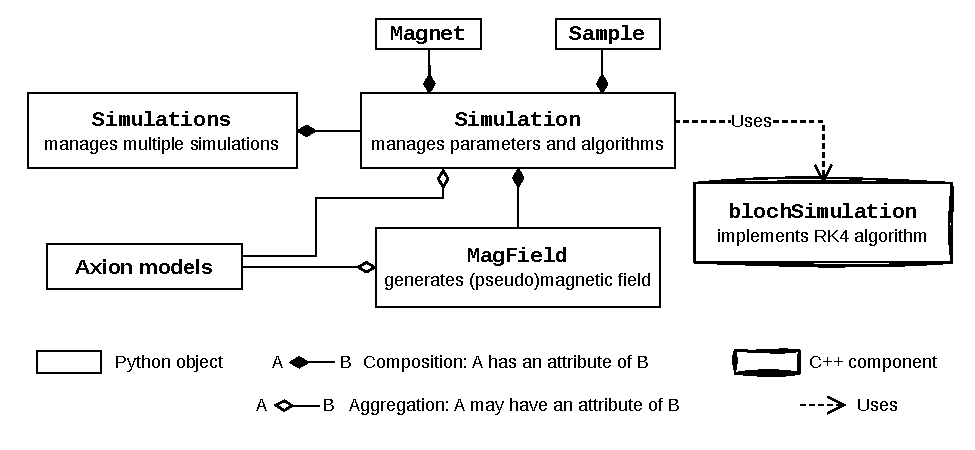
\includegraphics[scale=0.95]{figures/diagram_v1.1.drawio.pdf}}
    \caption{Architecture of \axionbloch{}. Each \texttt{Simulation} instance imports parameters from \texttt{Magnet}, \texttt{Sample}, and \texttt{MagField} instances. For axion simulations, axion-model objects are required both for \texttt{Simulation} to configure the simulation and for \texttt{MagField} to generate the pseudomagnetic field. \texttt{Simulations} manages one or multiple \texttt{Simulation} instances. Numerical integration is performed via the \texttt{blochSimulation} API, which provides Python access to the underlying C++ implementation. 
    }
    \label{fig:architecture}
\end{figure*}

On the Python side, classes \texttt{Sample}, \texttt{Magnet}, and \texttt{MagField} encapsulate the relevant experimental parameters, including sample relaxation times, magnetic field strength and homogeneity. 
The axion field models are implemented by dedicated classes, such as \texttt{MilkyWayAxionHalo}, which carry the properties of the axion fields. Together with the method \texttt{MagField.setAxionFields()}, the pseudomagnetic fields can be generated. 
Different axion models can be incorporated as separate classes without modifying the simulation framework. 
Simulation is handled within the \texttt{axionbloch.SimuTools} module. 
In particular, the classes \texttt{Simulation} and \texttt{Simulations} manage the interaction between experimental configurations and axion field models, organizing the parameters and execution of single or multiple simulation runs. 

The RK4 algorithm is implemented in a dedicated C++ library. 
% This library is more efficient compared to a pure Python implementation. 
The application programming interface (API) for this library is \texttt{blochSimulation}. 
This C++ backend is interfaced with Python using \texttt{pybind11},\footnote{\url{http://pybind11.readthedocs.io/}} enabling cooperation between high-level Python workflow management and low-level efficient numerical computation. 

\subsection{Calibration}
\label{sec:calibration}

% \subsection{Examples}
% \label{sec:examples}

Accurate calibration is essential to ensure that the simulated signals reliably reflect the underlying physical system and can be compared with experimental observables. 
In particular, calibration examines the correspondence between the NMR signal and model parameters, including magnetic fields, nuclear spin gyromagnetic ratio $\gamma$ and relaxation times ($T_1$, $T_2$ and $T_2^*$). 
It allows one to verify the correctness and stability of the numerical implementation. 
In this section, examples of calibration simulations are presented along with theoretical predictions, demonstrating the methodology of calibration. 
A quantitative analysis is included at the end of the section. 
% These ensure that the simulations produce quantitatively accurate results. 
For the examples in the section, an ethanol sample and an axial bias field $\mathbf{B_{0}} = B_0 \mathbf{\hat{e}}_z$ are used. 

\subsubsection{Pulsed-NMR: Free Decay and Spin Echo}
\label{sec:pNMR}
In the pulsed-NMR calibration, one $\SI{90}{\degree}$ and one $\SI{180}{\degree}$ magnetic-field pulse are applied in the simulation. 
The magnetization is expected to\,\cite{CPMG, Abragam1961_NuclearMagnetism}:
\begin{itemize}
    \item oscillate at the Larmor frequency;
    \item be tipped by $\SI{90}{\degree}$ to the x-y plane by the $\SI{90}{\degree}$ pulse;
    \item free decay with relaxation time $T_2^*$ in the absence of pulses;
    \item refocus (echo) after $\SI{180}{\degree}$ pulses; 
    \item show decaying amplitude of echoes with relaxation time $T_2$.
\end{itemize}
The behaviors described above can be found in the calibration example illustrated in \cref{fig:calibration_T2_T2star}\,(a), indicating correct simulation behavior. 
With such benchmarks, magnetic pulses, Larmor precession, and transverse relaxations ($T_2$ and $T_2^*$) can be calibrated. 

\begin{figure*}
    \centering
    
\includegraphics{figures/SpinEcho_and_CW.pdf}
    \caption{Simulated magnetic fields in x and y directions (upper row) and induced NMR signals (lower row). The magnetizations plotted are normalized by equilibrium magnetization. (a) After $\SI{90}{\degree}$ and $\SI{180}{\degree}$ magnetic-field pulses in x-y plane, free decay (relaxation time $T_2^*$) and echo signals (relaxation time $T_2$) are generated. (b) Excited by a weak CW magnetic field, the NMR signals increase with $\gamma B T_2^* (1 - e^{-t/T_2^*})$, where $B = \sqrt{B_x^2+B_y^2}$ is the magnitude of the excitation. 
    \HB{In (a)-top, why is there a nonzero $B_y$ component at the pulses?}
    \YZ{This indicates the orientation of the magnetic pulse. The pulse is like $a B_x + b B_y$. }
    }
    \label{fig:calibration_T2_T2star}
\end{figure*}


\subsubsection{Continuous-Wave NMR}
\label{sec:CW_NMR}
In the continuous-wave (CW) NMR calibration, an oscillating magnetic field is applied. 
When the magnetic field strength $B$ is weak ($\gamma B T_2^*\ll 1$) and on resonance, the transverse magnetization grows with $\gamma B T_2^* (1 - e^{-t/T_2^*})$\,\cite{Abragam1961_NuclearMagnetism}.
One such example is illustrated in \cref{fig:calibration_T2_T2star}\,(b). 
% The simulation goes as expected. 
The simulation produces the expected results.
% \HB{The simulation produces the expected results.}
With such benchmarks, the Larmor precession and $T_2^*$ relaxation can be calibrated. 

\subsubsection{Hyperpolarized sample}
\label{sec:hyperpol}

To achieve better sensitivity to the axion field, hyperpolarization is favored in experiments. Compared to thermal polarization at room temperature, hyperpolarization techniques can boost the polarization by orders of magnitude to the order of unity. 
The \axionbloch{} package handles the polarization by the \texttt{Sample} class. 
A \SI{1}{\%}-polarization ethanol sample is used as an example demonstrating the evolution of hyperpolarization due to the $T_1$ relaxation. 
At first ($t\ll T_1$), the polarization should exponentially decays with time constant $T_1$, until it reaches equilibrium after many $T_1$. 
As can be seen in \cref{fig:calibration_T1_HP}, the simulated $T_1$ relaxation agrees with the expected behavior. 
More of such simulations can be applied in calibrating $T_1$ relaxation. 

\begin{figure}
    \centering
    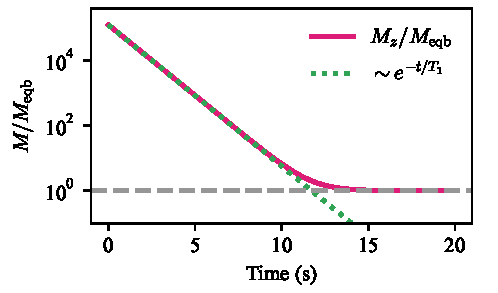
\includegraphics{figures/T1_hyperpolarized.pdf}
    \caption{
    Simulated $T_1$ relaxation of a hyperpolarized sample in a static bias field. The axial magnetization $M_z$ is normalized by the equilibrium magnetization $M_0$. 
    }
    \label{fig:calibration_T1_HP}
\end{figure}


\subsubsection{Quantitative evaluation}

The accuracy of simulations is evaluated by the discrepancy between the theoretically expected magnetization and simulation results, characterized by
\begin{equation}
    \chi^2 = \dfrac{\sum |M_\mathrm{expected} - M_\mathrm{simu}|^2}{\sum |M_\mathrm{simu}|^2}
    \,. 
    \label{eq:chisq}
\end{equation} 
Here $M_\mathrm{expected}$ and $M_\mathrm{simu}$ are magnetization expected and simulated, respectively. 
$\sum$ denotes the sum over integration steps.
A well-calibrated simulation should give $\chi^2\ll 1$. 
Calibration scripts are stored in the test script set of \axionbloch{}. 
In each calibration, parameters such as Larmor frequency and relaxation times are varied over orders of magnitude to cover all possible cases in simulation.
The results of the calibrations are summarized in \cref{tab:calibration_summary}. 
The discrepancies are generallly small ($\chi^2 < 10^{-4}$).
If a certain simulation precision is required, the $\chi^2$ value serves as a quantitative reference. 
\begin{table*}
    \caption{Summary of calibrations.
    Parameters were swept over orders of magnitude to cover all simulation regimes. 
    \HB{all realistic regimes? For example, up to the highest available superconducting magnet fields? Maybe it should somewhere be mentioned (near the hamiltonians) that this package is currently not capable of simulating ZULF phenomena, such as j-coupling?}
    \YZ{ZULF NMR is not really covered. I will include more information about the regimes. }
    $\chi^2$ is defined in \cref{eq:chisq}; $\chi^2\ll 1$ indicates a well-calibrated simulation.
    Here $\nu_L$ stands for Larmor frequency, determined by the bias magnetic field and $\nu_\mathrm{RCF}$ is RCF frequency. 
    Technical details of the calibrations can be found in the test script set. 
    Note that the integration step size is chosen to be $T_2^* / 500$. 
    Discrepencies can be even smaller by using smaller step size at the cost of runtime consumption. 
    }
    \label{tab:calibration_summary}
    \begin{ruledtabular}
    \begin{tabular}{lllll}
        \parbox[t]{2.5cm}{\raggedright\textbf{Calibration}} &
        \parbox[t]{3.5cm}{\raggedright\textbf{Parameters calibrated}} &
        \parbox[t]{3.0cm}{\raggedright\textbf{Varied parameters}} &
        \parbox[t]{1.2cm}{\raggedright $\bm{\chi^2}$} &
        \parbox[t]{5.0cm}{\raggedright\textbf{Dominant source of error}} \\[8pt]
        \hline
        \parbox[t]{2.5cm}{\raggedright Pulsed NMR: free decay} &
        \parbox[t]{3.5cm}{\raggedright Pulse amplitude, $\nu_L$, $T_2^*$, $T_2$} &
        \parbox[t]{3.0cm}{\raggedright $\nu_\mathrm{RCF}$} &
        \parbox[t]{1.2cm}{\raggedright $<10^{-4}$} &
        \parbox[t]{5.0cm}{\raggedright Finite number of steps for hard pulses. } \\[8pt]
        \parbox[t]{2.5cm}{\raggedright CW-NMR} &
        \parbox[t]{3.5cm}{\raggedright $\nu_L$ and $T_2^*$} &
        \parbox[t]{3.0cm}{\raggedright $\nu_\mathrm{RCF}$} &
        \parbox[t]{1.2cm}{\raggedright $<10^{-5}$}  &
        \parbox[t]{5.0cm}{\raggedright Finite integration step size.  } \\[8pt]
        \parbox[t]{2.5cm}{\raggedright $T_1$ relaxation} &
        \parbox[t]{3.5cm}{\raggedright $T_1$} &
        \parbox[t]{3.0cm}{\raggedright $\nu_\mathrm{RCF}$, $\nu_L$, initial polarization} &
        \parbox[t]{1.2cm}{\raggedright $<10^{-7}$}  & 
        \parbox[t]{5.0cm}{\raggedright Finite integration step size. } \\
    \end{tabular}
    \end{ruledtabular}
\end{table*}


\subsection{Axion Simulation}
\label{sec:simulation}

Similar to the calibration examples, axion-induced NMR signals were generated by solving the Bloch equations with the axion-induced pseudomagnetic field as part of the effective magnetic field. 
An example of a commonly considered model -- axion constituting the Milky Way galactic dark matter halo\,\cite{Evans2019_SHMRefined,Gramolin2022Feb_SpectralSignatures} is implemented in the class \texttt{MilkyWayAxionHalo}. 
In this model, the axion field is treated as an oscillating field with a frequency determined by the axion mass, and a linewidth (characterizing the stochasticity) determined by the velocity dispersion of the virialized dark matter halo. 
The sample is chosen to be \ch{^{129}Xe}, polarized to $\SI{50}{\%}$ initially, and the bias field is applied along the z direction. 
The details of the simulation configuration can be found in the code example in \cref{code:axion_example}. 
Readers are referred to \cref{fig:architecture} which illustrates the relationship between the objects in the code example. 
The simulated pseudomagnetic fields and the amplitude of the induced transverse magnetization are shown in \cref{fig:MilkyWayAxionHalo}, in which the signal is seen to increase with time at the beginning of the simulation due to the axion field gradient, and then decay due to the $T_1$ relaxation. 
The efficiency of the simulation is limited by time consumption for the numerical integration of the Bloch equations. 
The total number of integration steps can be found by
\begin{align}
    N &= \text{\texttt{Simulation.rate}} \times \text{\texttt{Simulation.duration}} \nonumber\\
    &\quad \times \text{\texttt{MagField.numFields}} \times \text{\texttt{Magnet.numPt}}\,,
\end{align}
where \texttt{Simulation.rate} is the rate of the simulation, \texttt{Simulation.duration} is the duration of the simulation, \texttt{MagField.numFields} is the number of random pseudomagnetic fields generated to account for the stochasticity of the axion field, and \texttt{Magnet.numPt} is the number of bias fields sampled to account for the inhomogeneity of the bias field.
For the example in \cref{code:axion_example}, the total number of integration steps is \SI{4.064e9}{}, and the runtime is \SI{10}{\s} on a personal computer (CPU: Intel\textsuperscript{\textregistered} Core\textsuperscript{\texttrademark} Ultra 7 155H; base speed: 1.40\,GHz). 
Such moderate runtime allows users to explore different parameter regimes with many simulations. 

\begin{figure}
\center
\fbox{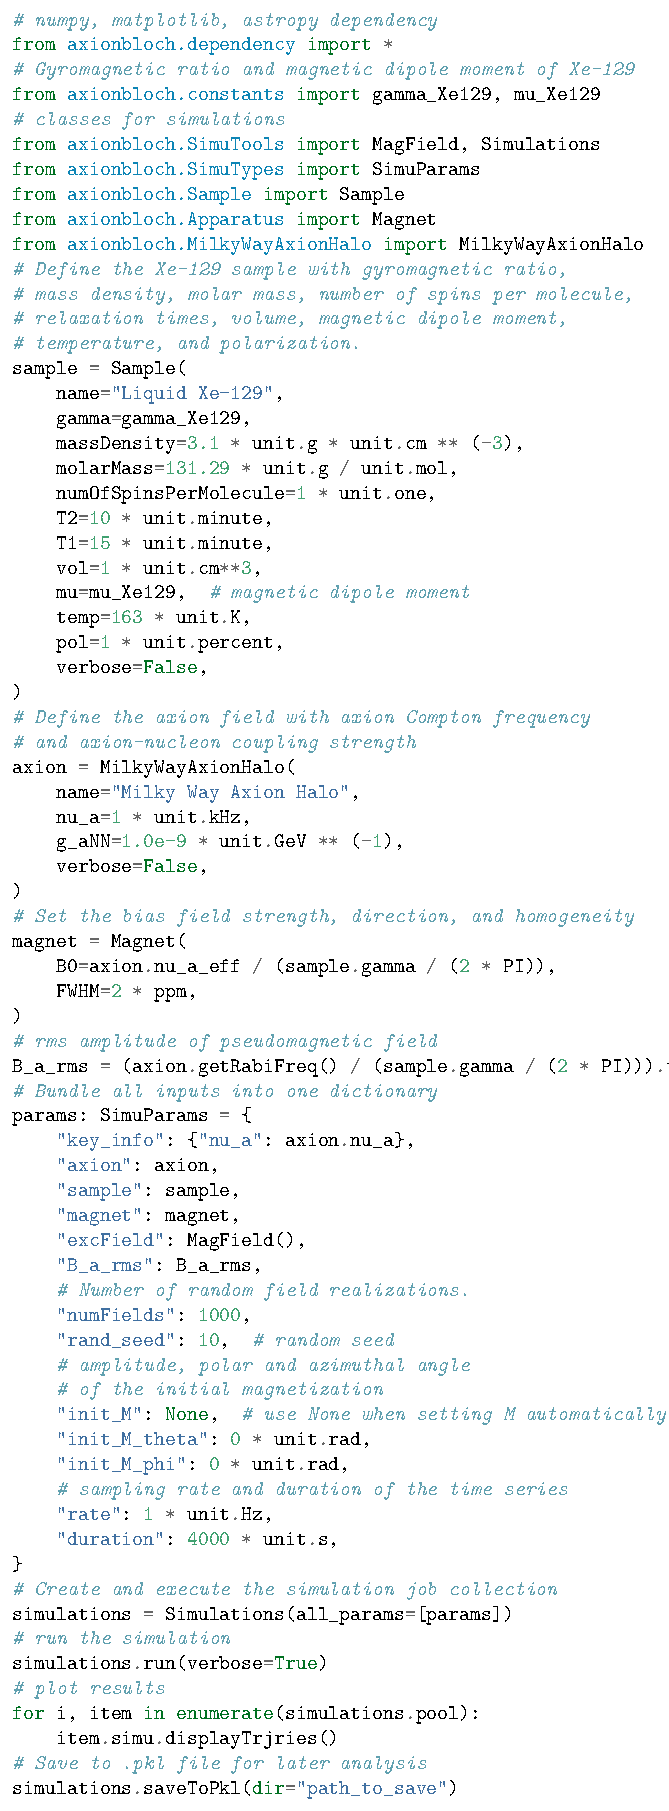
\includegraphics[scale=0.7,clip]{figures/axion_example.pdf}}
% \vspace{0.1in}
\caption{Example code of an axion simulation.}
\label{code:axion_example}
\end{figure}

% \begin{figure}
%     \centering
%     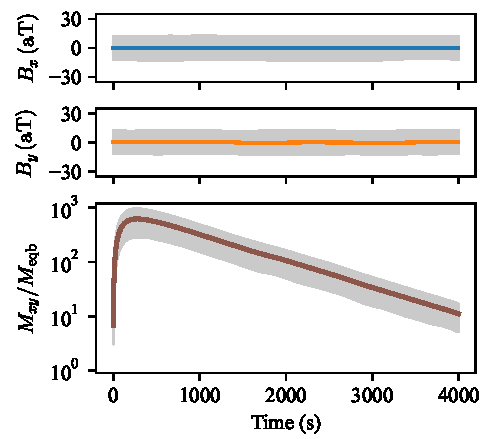
\includegraphics[width=\linewidth]{figures/MilkyWayAxionHalo-1000.pdf}
%     \caption{Simulation of local virialized axion dark matter halo. From top to bottom: pseudomagnetic fields in the transverse plane ($B_x$ and $B_y$) and the transverse magnetization induced ($M_{xy}$). To account for the stochasticity, generated 1000 pseudomagnetic fields were generated. The solid lines indicate the mean of these 1000 $B_x$, $B_y$, and $M_{xy}$, while the gray shadows indicate $\pm \sigma$ (standard deviation) range. The sample for the simulations was assumed to be polarized to $\SI{50}{\%}$ initially. 
%     }
%     \label{fig:MilkyWayAxionHalo}
% \end{figure}

\begin{figure*}
    \centering
    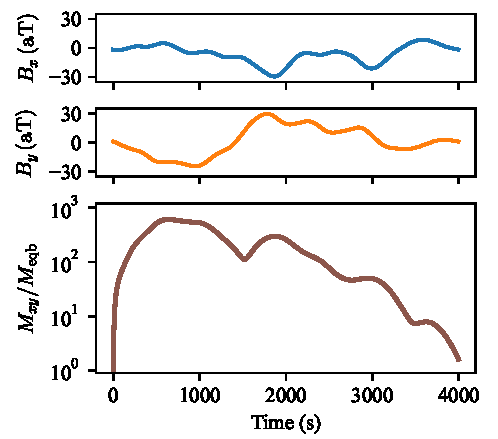
\includegraphics[width=0.49\linewidth]{figures/MilkyWayAxionHalo-1.pdf}
    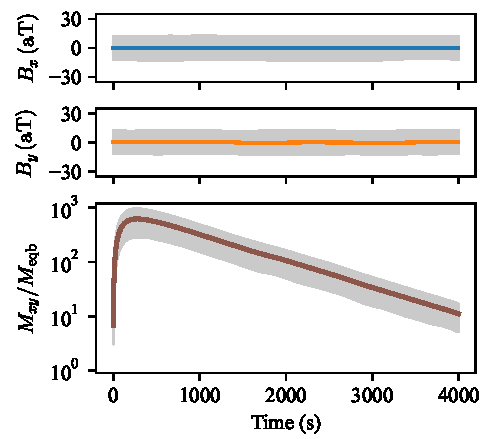
\includegraphics[width=0.49\linewidth]{figures/MilkyWayAxionHalo-1000.pdf}
    \caption{Simulations of local virialized axion dark matter halo. From top to bottom: pseudomagnetic fields in the transverse plane ($B_x$ and $B_y$) and the transverse magnetization induced ($M_{xy}$). Left: one single simulation. Right: 1000 simulations to account for the stochasticity. The solid lines indicate the value (left column) or mean value (right column) of $B_x$, $B_y$, and $M_{xy}$, while the gray shadows indicate $\pm \sigma$ (standard deviation) range. The sample for the simulations was assumed to be polarized to $\SI{50}{\%}$ initially.
    }
    \label{fig:MilkyWayAxionHalo}
\end{figure*}



% \subsubsection{Earth-bound axionlike dark matter}

% [should this example be mentioned?]


%-----------------------
\section{Development}
\label{sec:dev-approach}
%-----------------------

% Version Control
Development of \axionbloch{} is managed using \texttt{git},\footnote{\url{http://git-scm.com}} with the code hosted on a public GitHub repository.\footnote{\url{https://github.com/Yuzhe98/AxionBloch}} 
Changes to the main codebase follow a \textit{pull request} workflow, allowing contributions to be reviewed before being merged. Users can participate by forking the repository, making modifications in their fork, and submitting pull requests for review by the developers.
As \axionbloch{} is intended as a collaborative resource, user contributions and suggestions are encouraged and appreciated. 

% Automated Testing with pytest
\axionbloch{} includes a suite of automated tests to ensure correctness and reliability. 
The tests are implemented using the \texttt{pytest} framework,\footnote{\url{https://docs.pytest.org/}} which allows for calibration of physical processes and testing of functions, classes, and modules. 
The test suite covers core functionalities such as:
\begin{itemize}
    \item initialization and manipulation of classes; 
    \item numerical integration of the Bloch equations;
    \item magnetic fields and relaxations;
    \item handling of each axion field configuration.
\end{itemize}
Tests can be executed locally. In the future, tools may be added for online testing considering the demand of testing. 
Regular execution of the test suite ensures that new changes do not introduce regressions, maintaining the stability and correctness of the package.

% documentation
Documentation for \axionbloch{} is available on Read the Docs.\footnote{\url{http://axionbloch.readthedocs.io}}
It is built using \texttt{Sphinx}\footnote{\url{http://www.sphinx-doc.org}} and provides detailed explanations of the API, along with instructions for installation, configuration, and usage.

% Future
As numerous new axion field models and experiments are emerging, the functionality of \axionbloch{} may extend so that it can be a tool for updating our knowledge of the induced spin dynamics. 

%-----------------------
\section{Conclusions}
\label{sec:conclusions}
%-----------------------

\axionbloch{} has been presented as a framework for simulating spin dynamics induced by magnetic fields or axion fields under a variety of physical scenarios. 
The package adopts SI units so that the inputs and outputs are directly comparable to experimental parameters and observables. 
Numerical integration of the Bloch equations is performed using a fourth-order Runge--Kutta method in the rotating coordinate frame, enabling stable and efficient simulation. 
Comprehensive calibrations have been performed to ensure the accuracy of the simulations.
An example simulation of axion-induced signals from a local virialized axion dark matter halo is presented to demonstrate the package's capabilities. 

By providing an open-source, well-documented, and tested tool, \axionbloch{} aims to facilitate the study of axion-induced spin dynamics in precision measurement experiments and to serve as a platform for further method development and incorporation of new axion models.

Note that this package can be of interest to the NMR community for its applications in, for example, educational purposes. 
For example, students can specify pulse sequences for the simulation and see the visualized simulation results. 

%-----------------------
\section*{Data Availability}
\label{sec:data-availability}
%-----------------------
The data and code that generate this manuscript are available at \url{
https://github.com/Yuzhe98/AxionBloch-paper}. 

\begin{acknowledgments}

The author acknowledges helpful discussion with Hendrik Bekker, Dmitry Budker and Alexander Sushkov. 
The author is grateful to the communities supporting the open-source software and tools: \texttt{git}, \texttt{NumPy}, 
\texttt{SciPy}\footnote{\url{https://docs.scipy.org/}}\,\cite{Virtanen2020_SciPy}, 
\texttt{matplotlib}\footnote{\url{https://matplotlib.org/}}, 
\texttt{astropy}, 
\texttt{pybind11}, 
\texttt{IPython}\footnote{\url{https://ipython.org/}}\,\cite{Perez2007_IPython}, 
\texttt{Jupyter}\footnote{\url{https://jupyter.org/}}\,\cite{Granger2021_Jupyter}, 
\texttt{pytest}, 
\texttt{Sphinx}, 
GitHub\footnote{\url{https://github.com/}} 
and 
Read the Docs\footnote{\url{https://about.readthedocs.com/}}. 
This work has been supported by the Cluster of Excellence ``Precision Physics, Fundamental Interactions, and Structure of Matter'' (PRISMA++ EXC 2118/2) funded by the
German Research Foundation (DFG) within the German Excellence Strategy (Project ID 390831469).

\end{acknowledgments}

% \section*{Author Contribution Statement}


% Yuzhe Zhang: Conceptualization, Software, Visualization, Writing -- original draft and Writing -- review \& editing

% Dmitry Budker: Funding acquisition, Supervision,  Writing -- review \& editing

% \textbf{Author contribution roles and definitions}

% \begin{description}

% \item[Conceptualization]
% Ideas; formulation or evolution of overarching research goals and aims.

% \item[Data curation]
% Management activities to annotate (produce metadata), scrub data, and maintain research data (including software code, where necessary for interpreting the data itself) for initial use and later re-use.

% \item[Formal analysis]
% Application of statistical, mathematical, computational, or other formal techniques to analyze or synthesize study data.

% \item[Funding acquisition]
% Acquisition of the financial support for the project leading to this publication.

% \item[Investigation]
% Conducting a research and investigation process, specifically performing the experiments or data/evidence collection.

% \item[Methodology]
% Development or design of methodology; creation of models.

% \item[Project administration]
% Management and coordination responsibility for the research activity planning and execution.

% \item[Resources]
% Provision of study materials, reagents, materials, laboratory samples, instrumentation, computing resources, or other analysis tools.

% \item[Software]
% Programming, software development; designing computer programs; implementation of the computer code and supporting algorithms; testing of existing code components.

% \item[Supervision]
% Oversight and leadership responsibility for the research activity planning and execution, including mentorship external to the core team.

% \item[Validation]
% Verification, whether as a part of the activity or separate, of the overall replication or reproducibility of results, experiments, and other research outputs.

% \item[Visualization]
% Preparation, creation, and/or presentation of the published work, specifically visualization or data presentation.

% \item[Writing -- original draft]
% Preparation, creation, and/or presentation of the published work, specifically writing the initial draft (including substantive translation).

% \item[Writing -- review \& editing]
% Preparation, creation, and/or presentation of the published work by members of the original research group, specifically critical review, commentary, or revision, including pre- or post-publication stages.

% \end{description}

% \appendix

% \include{appendix.tex}

\bibliographystyle{unsrt}
\bibliography{references}% Produces the bibliography via BibTeX.

\end{document}